\documentclass[tikz,border=3pt]{standalone}
\usepackage[utf8]{inputenc}
\usepackage[T1]{fontenc}
\usepackage{lmodern}
\renewcommand{\familydefault}{\sfdefault}
\usepackage{sansmath}\sansmath
\usepackage{chemfig}
\usepackage{pgfplots}\pgfplotsset{compat=1.18,/pgf/number format/use comma,/pgf/number format/1000 sep={.}}
\usetikzlibrary{arrows.meta,calc,positioning,decorations.pathmorphing,patterns}
% paleta del sitio
\definecolor{nar}{HTML}{E8680C}\definecolor{narc}{HTML}{FFB35C}\definecolor{hielo}{HTML}{FFF3E8}
\definecolor{tinta}{HTML}{1D1D1F}\definecolor{gris}{HTML}{6E6E73}\definecolor{lila}{HTML}{7C5CF0}
\definecolor{azul}{HTML}{2F6FD6}\definecolor{menta}{HTML}{17A673}\definecolor{coral}{HTML}{E8342A}
\begin{document}
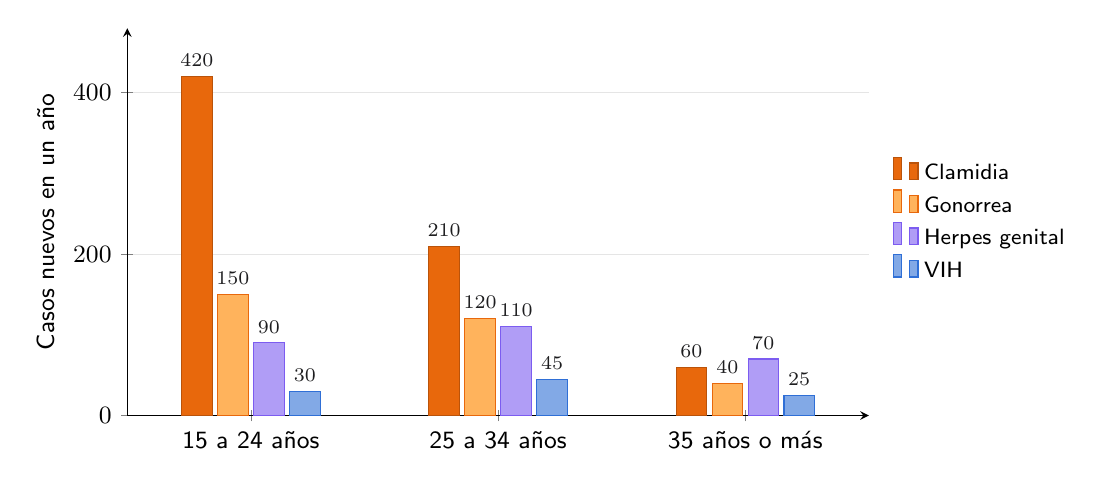
\begin{tikzpicture}[font=\small]
\begin{axis}[width=11cm,height=6.5cm,ybar,bar width=11pt,ymin=0,ymax=480,xmin=0.5,xmax=3.5,axis lines=left,
 xtick={1,2,3},xticklabels={15 a 24 años,25 a 34 años,35 años o más},ylabel={Casos nuevos en un año},
 ymajorgrids,grid style={gray!20},nodes near coords,every node near coord/.append style={font=\scriptsize,text=tinta},
 legend cell align=left,legend style={draw=none,fill=none,at={(1.02,0.5)},anchor=west,font=\footnotesize}]
\addplot[fill=nar,draw=nar!80!black] coordinates {(1,420)(2,210)(3,60)};
\addlegendentry{Clamidia}
\addplot[fill=narc,draw=nar] coordinates {(1,150)(2,120)(3,40)};
\addlegendentry{Gonorrea}
\addplot[fill=lila!60,draw=lila] coordinates {(1,90)(2,110)(3,70)};
\addlegendentry{Herpes genital}
\addplot[fill=azul!60,draw=azul] coordinates {(1,30)(2,45)(3,25)};
\addlegendentry{VIH}
\end{axis}
\end{tikzpicture}
\end{document}
